\documentclass[journal,12pt,twocolumn]{IEEEtran}
\usepackage{amsthm}
\usepackage{graphicx}
\usepackage{mathrsfs}
\usepackage{txfonts}
\usepackage{stfloats}
\usepackage{pgfplots}
\usepackage{cite}
\usepackage{cases}
\usepackage{mathtools}
\usepackage{caption}
\usepackage{enumerate}	
\usepackage{enumitem}
\usepackage{amsmath}
\usepackage[utf8]{inputenc}
\usepackage[english]{babel}
\usepackage{multicol}
%\usepackage{xtab}
\usepackage{longtable}
\usepackage{multirow}
%\usepackage{algorithm}
%\usepackage{algpseudocode}
\usepackage{enumitem}
\usepackage{mathtools}
\usepackage{gensymb}
\usepackage{hyperref}
%\usepackage[framemethod=tikz]{mdframed}
\usepackage{listings}
    %\usepackage[latin1]{inputenc}                                 %%
    \usepackage{color}                                            %%
    \usepackage{array}                                            %%
    \usepackage{longtable}                                        %%
    \usepackage{calc}                                             %%
    \usepackage{multirow}                                         %%
    \usepackage{hhline}                                           %%
    \usepackage{ifthen}                                         %%
  \providecommand{\nCr}[2]{\,^{#1}C_{#2}}
  \providecommand{\nPr}[2]{\,^{#1}P_{#2}}
  \lstset{
%language=C,
frame=single, 
breaklines=true,
columns=fullflexible
}

\title{Assignment 5
\\Probability and Random Variables }
\author{Swati Mohanty (EE20RESCH11007) }
\date{March 2021}

\begin{document}

\maketitle


\section{Problem}
In a game, a man wins a rupee for a six and
loses a rupee for any other number when a
fair die is thrown. The man decided to throw
a die thrice but to quit as and when he gets a
six. Find the expected value of the amount he
wins / loses.

\section{Solution}
Let X denote the random variable of winning/losing in the game.
\\P(X = 1)= P(win) = getting a 6 on rolling a fair die.
\\P(X = 0)= P(loss) = getting a 6 on rolling a fair die.
\\P(X = 1) = p =$\frac{1}{6}$  = 0.167
\\P(X = 0) = 1-p = $\frac{5}{6}$ = 0.833
\\Let Y denote the random variable of winning the game in Nth trial, there can be 4 possible cases with the following probability:
\\(i)Wins in first throw:\begin{align}
    P(Y=1) = p = 0.167
\end{align}
\\(ii)Wins in the second throw :\begin{align}
    P(Y=2) = (1-p)\times p = 0.139
\end{align}
\\(ii)Wins in the third throw :\begin{align}
    P(Y=3) = (1-p)\times(1-p)\times p = 0.107
\end{align}
\\(ii)Does not wins in any throw :\begin{align}
    P(Y=3) = (1-p)\times(1-p)\times (1-p) = 0.596
\end{align}

Net amount = P(Y=1)\times1 +P(Y=1)\times(-1+1) + P(Y=1)\times(-1-1+1) + P(Y=1)\times(-1-1-1) = -1.73



\\The probabilities were simulated using the python code.
\begin{figure}[h]
\renewcommand{\theenumi}{1}
\centering
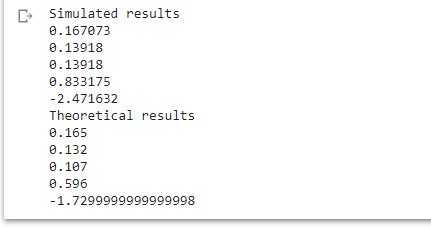
\includegraphics[ width=\columnwidth , height =5cm]{unif.PNG}
\caption{Simulation for tossing a fair coin  }
\label{Fig:1}


\end{figure}

\textbf{Download python code from here}\\
\begin{lstlisting}
https://github.com/Swati-Mohanty/AI5002/blob/main/Assignment_5/codes/die.py
\end{lstlisting}
\textbf{Download latex code from here-}\\
\begin{lstlisting}
https://github.com/Swati-Mohanty/AI5002/blob/main/Assignment_5/codes/assignment5.tex
\end{lstlisting}

\end{document}
